%!TEX root = main.tex

\newpage
\section{Реализация ОА}

Для реализации цифрового автомата использовалась САПР <<Альтера>> Max+plus II.

\subsection{Реализация ОА${}_1$}

\begin{figure}[H]
	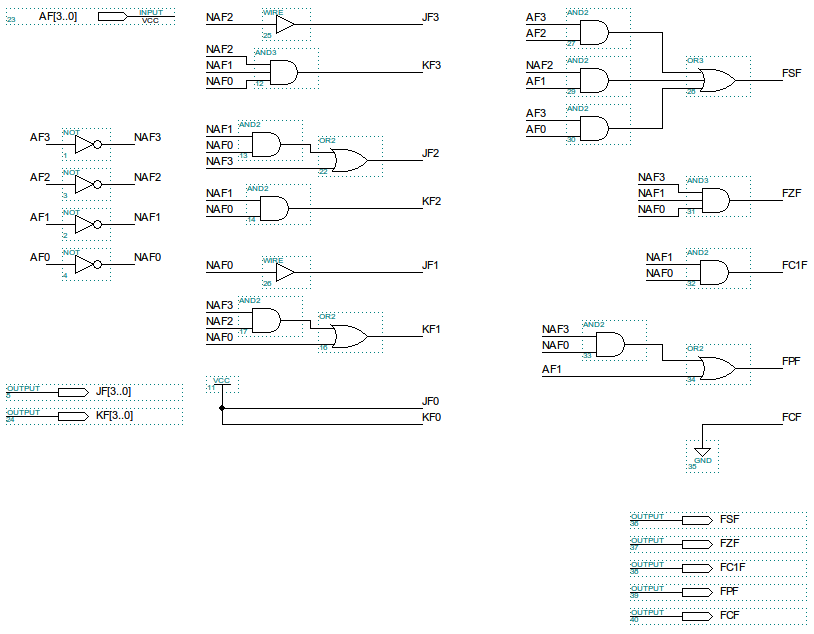
\includegraphics[scale=0.6]{images/altera/oa10_logic.png}
	\caption{Схема ОА$^{(0)}_{1}$}
	\label{figure:oa10log}
\end{figure}

\begin{figure}[H]
	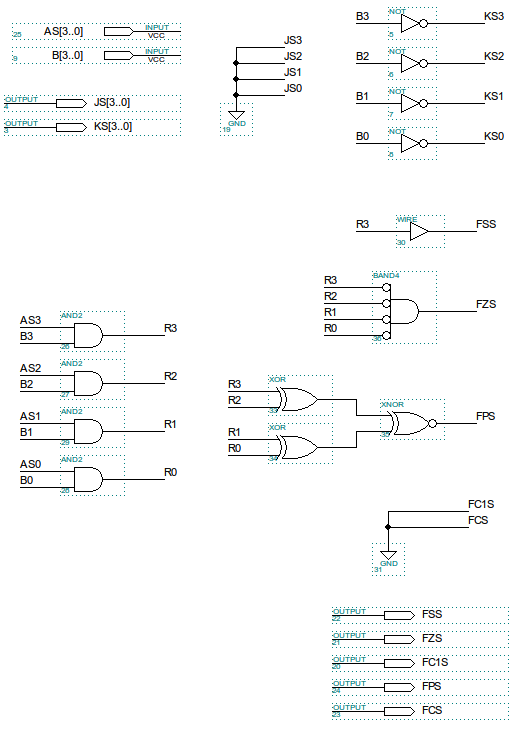
\includegraphics[scale=0.6]{images/altera/oa11_logic.png}
	\caption{Схема ОА$^{(1)}_{1}$}
	\label{figure:oa11log}
\end{figure}

\begin{figure}[H]
	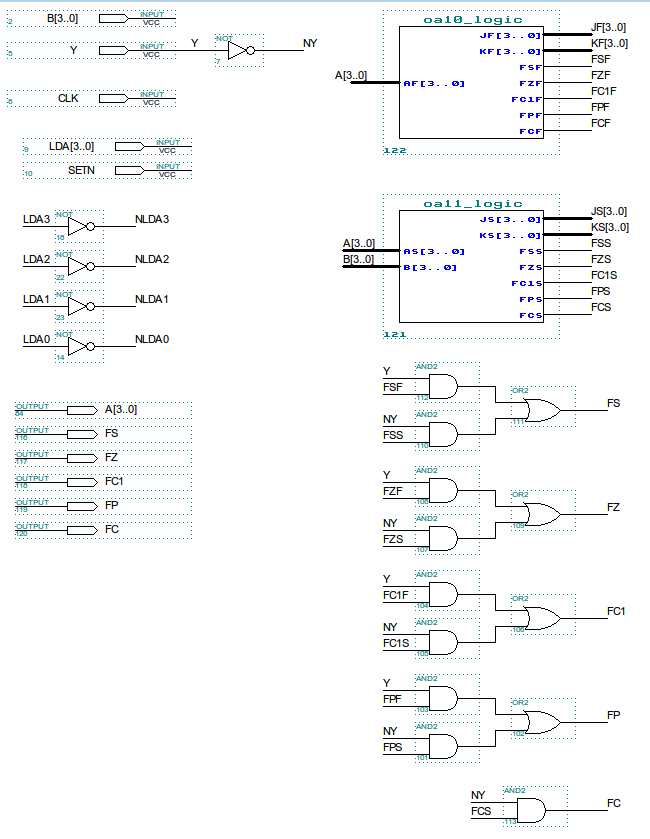
\includegraphics[scale=0.6]{images/altera/oa1_1.png}
	\caption{Cхема ОА$_{1}$ (начало)}
	\label{figure:oa1-1log}
\end{figure}

\begin{figure}[H]
	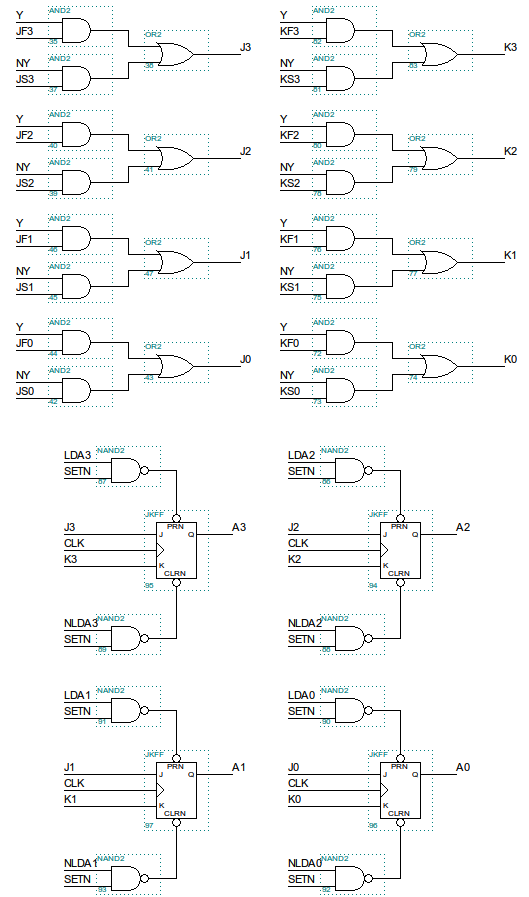
\includegraphics[scale=0.6]{images/altera/oa1_2.png}
	\caption{Cхема ОА$_{1}$ (окончание)}
	\label{figure:oa1-2log}
\end{figure}


\clearpage
\subsection{Реализация ОА${}_2$}

\begin{figure}[H]
	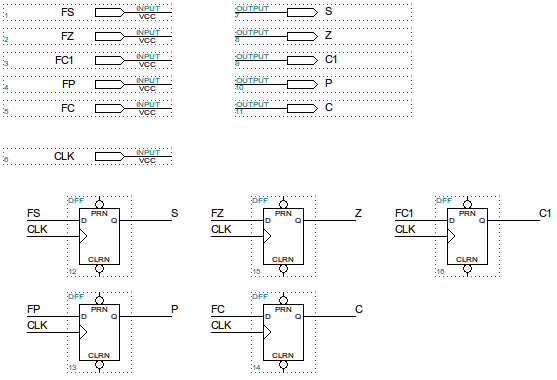
\includegraphics[scale=0.6]{images/altera/oa2.png}
	\caption{Cхема ОА$_{2}$}
	\label{figure:oa2log}
\end{figure}

\subsection{Реализация ОА}

\begin{figure}[H]
	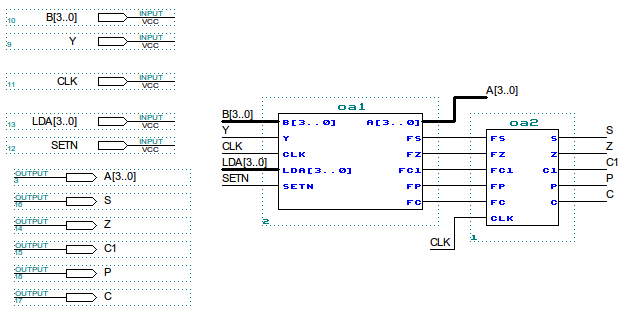
\includegraphics[scale=0.6]{images/altera/oa.png}
	\caption{Cхема ОА}
	\label{figure:oalog}
\end{figure}

\newpage
\section{Моделирование ОА}

\subsection{Методика моделирования}

Процесс моделирования данного автомата был разделен на 3 этапа:
\begin{itemize}
	\item Моделирование ОА$_1$. Целью моделирования ОА1 является проверка правильности выполнении операций, проверка формирования значений логических функций признаков $f_S$, $f_Z$, $f_{C'}$, $f_P$, $f_C$. 
	\item Моделирование ОА$_2$. На данном этапе осуществляется проверка правильности записи значений признаков $S$, $Z$, $C'$, $P$, $C$.
	\item Моделирование ОА. На данном этапе осуществлялась проверка правильности взаимодействия автоматов ОА$_1$ и ОА$_2$. 
\end{itemize}

\subsection{Моделирование ОА$_1$}

Описание сигналов:
\begin{itemize}	
	\item CLK --- импульс тактовой частоты,
	
	\item LDA ---  шина установки состояния автомата,
	
	\item SETN --- сигнал, переводящий автомат в состояние с шины LDA,
	
	\item Y --- сигнал, определяющий выполняемую операцию,
	
	\item A --- состояние автомата,
	
	\item FS --- признак знака,
	
	\item FZ --- признак нуля,
	
	\item FP --- признак паритета,
	
	\item FC --- признак переноса,
	
	\item FC1 --- признак вспомогательного переноса.
\end{itemize}


\subsubsection{Моделирование арифметической операции}

На вход ОА1 подаются следующие сигналы:
\begin{itemize}
	\item сигнал кода операции \texttt{Y = 1},
	\item сигнал \texttt{LDA = 0011}$_2$, соответствующий числу 3h (первому разрешенному состоянию),
	\item импульс \texttt{SETN}, соответствующий переходу автомата в состояние с шины \texttt{LDA},
	\item импульсы тактовой частоты \texttt{CLK}.
\end{itemize}
 
Корректной работе автомата соответствуют значения на выходах, приведенные в таблице \ref{table:oa10test}.

Временная диаграмма результатов моделирования представлена на рисунке \ref{figure:oa10test}.

\clearpage
\begin{table}[H]
	\centering
	\caption{Ожидаемые результаты моделирования операции $A \leftarrow A - 1$}
	\label{table:oa10test}
	\begin{tabular}{|l|*{7}{c|}{r|}} \hline
		A(t) & A(t+1) & FS & FZ & FC1 & FP & FC \\ \hline
		0011 & 1100 & 1 & 0 & 0 & 1 & 0 \\ \hline
		1100 & 1011 & 1 & 0 & 1 & 0 & 0 \\ \hline
		1011 & 1010 & 1 & 0 & 0 & 1 & 0 \\ \hline
		1010 & 1001 & 1 & 0 & 0 & 1 & 0 \\ \hline
		1001 & 1000 & 1 & 0 & 0 & 0 & 0 \\ \hline
  		1000 & 0111 & 0 & 0 & 1 & 0 & 0 \\ \hline
		0111 & 0110 & 0 & 0 & 0 & 1 & 0 \\ \hline
		0110 & 0101 & 0 & 0 & 0 & 1 & 0 \\ \hline
		0101 & 0100 & 0 & 0 & 0 & 0 & 0 \\ \hline
		0100 & 0011 & 0 & 0 & 1 & 1 & 0 \\ \hline
	\end{tabular}
\end{table}

\begin{figure}[H]
	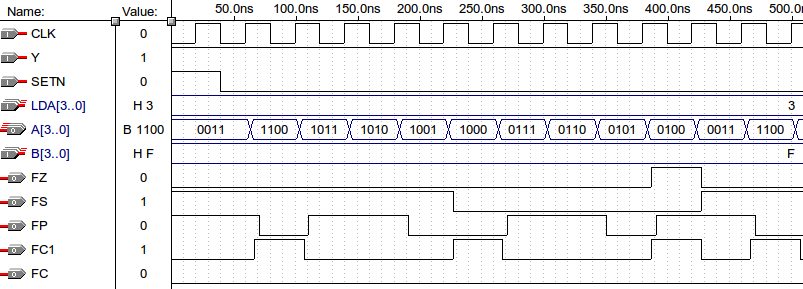
\includegraphics[scale=0.6]{images/altera/test10.png}
	\caption{Временная диаграмма результатов моделирования операции $A \leftarrow A - 1$}
	\label{figure:oa10test}
\end{figure}

Автомат циклически выполняет заданную операцию $A \leftarrow A - 1$ в коде в десятичной системе счисления в коде с избытком 3, вырабатывая сигналы от 3h до Ch в шестнадцатеричной системе счисления. Признаки устанавливаются в соответствии с таблицей \ref{table:oa10test}. То есть автомат функционирует в соответствии с заданием.

\clearpage
\subsubsection{Моделирование логической операции}

На вход ОА1 подаются следующие сигналы:
\begin{itemize}
	\item сигнал кода операции \texttt{Y = 0},
	\item сигналы \texttt{LDA}, соответствующие установке состояния),
	\item импульс \texttt{SETN}, соответствующий переходу автомата в состояние с шины \texttt{LDA},
	\item сигналы \texttt{B},
	\item импульсы тактовой частоты \texttt{CLK}.
\end{itemize}
 
Корректной работе автомата соответствуют значения на выходах, приведенные в таблице \ref{table:oa11test}.

Временная диаграмма результатов моделирования представлена на рисунке \ref{figure:oa11test}.

\begin{table}[H]
	\centering
	\caption{Ожидаемые результаты моделирования операции $A \leftarrow A \& B$}
	\label{table:oa11test}
	\begin{tabular}{|l|*{8}{c|}{r|}} \hline
		A(t) & B(t) & A(t+1) & FS & FZ & FC1 & FP & FC \\ \hline
		1010 & 0111 & 0010   & 0  & 0  & 0   & 0   & 0 \\ \hline
		0000 & 1001 & 0000   & 0  & 1  & 0   & 1   & 0 \\ \hline
		1111 & 0110 & 0110   & 0  & 0  & 0   & 1   & 0 \\ \hline
	\end{tabular}
\end{table}

\begin{figure}[H]
	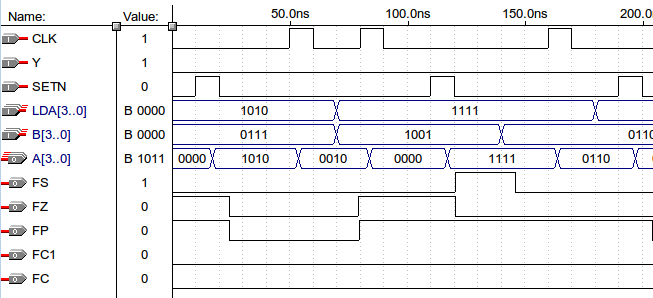
\includegraphics[scale=0.6]{images/altera/test11.png}
	\caption{Временная диаграмма результатов моделирования операции $A \leftarrow A \& B$}
	\label{figure:oa11test}
\end{figure}

Из временной диаграммы (Рисунок \ref{figure:oa11test}) видно, что автомат выполняет операцию $A \leftarrow A \& B$ в соответствии с ожидаемыми результатами таблицы \ref{table:oa11test}. 

Если с помощью схемы задания состояния записать в $A$ число 1010$_2$, а на шину $B$ подать сигнал, соответствующий числу 0111$_2$, то после прихода следующего импульса синхронизации $A = A \& B = 1010_2 \& 0111_2 = 0010_2$ и т.д. Признаки устанавливаются в соответствии с таблицей \ref{table:oa11test}. То есть автомат функционирует в соответствии с заданием.

\clearpage
\subsection{Моделирование ОА$_2$}

На триггеры Ds, Dz, Dc1, Dp, Dc подаются объединенные функции возбуждения fs, fz, fc, fp, fc1.

На выходах ОА$_2$ по положительному фронта синхроимпульса \texttt{CLK} записываются значения признаков S, Z, C1, P, C.

\begin{figure}[H]
	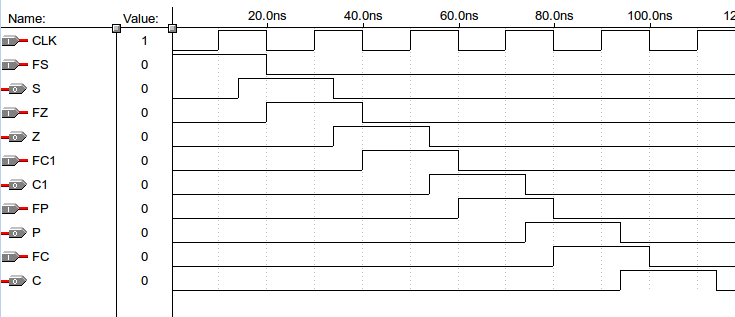
\includegraphics[scale=0.6]{images/altera/test2.png}
	\caption{Временная диаграмма результатов моделирования ОА$_2$}
	\label{figure:oa2test}
\end{figure}

Из диаграммы (Рисунок \ref{figure:oa2test}) видно, что схема работает корректно.

\clearpage
\subsection{Моделирование ОА}

На рисунках \ref{figure:oafin0test}, \ref{figure:oafin1test} приведены временные диаграммы (для y=0 и y=1 соответственно), иллюстрирующие работу автомата, состоящего из ОА$_1$ и ОА$_2$.

\begin{figure}[H]
	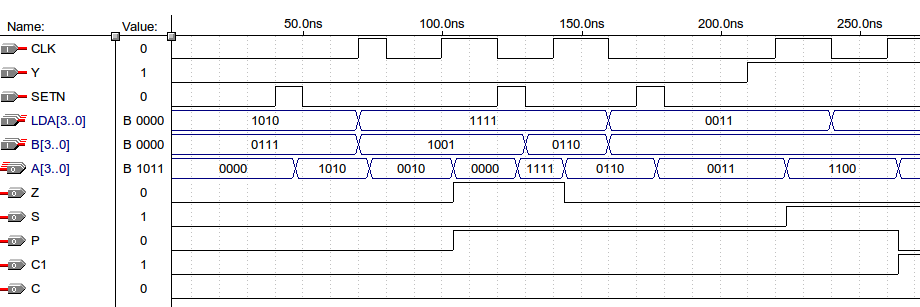
\includegraphics[scale=0.5]{images/altera/test_fin0.png}
	\caption{Временная диаграмма результатов моделирования ОА для y = 0}
	\label{figure:oafin0test}
\end{figure}

\begin{figure}[H]
	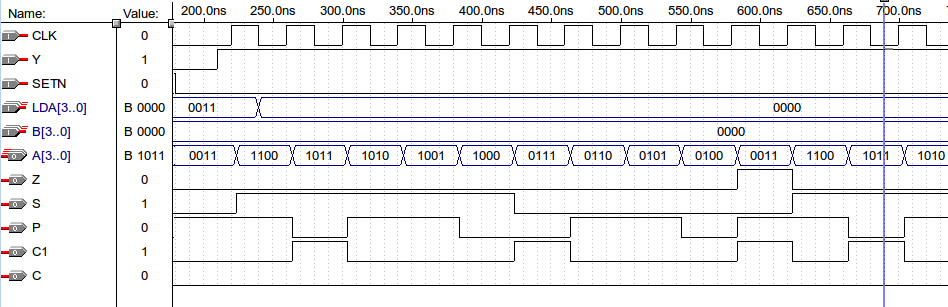
\includegraphics[scale=0.5]{images/altera/test_fin1.png}
	\caption{Временная диаграмма результатов моделирования ОА для y = 1}
	\label{figure:oafin1test}
\end{figure}

Из временных диаграмм видно, что результаты выполнения операций и признаки, совпадают со значениями из таблиц 2 и 5. То есть, автомат функционирует в соответствии с заданием.
